\documentclass[conference]{IEEEtran}

\usepackage[T1]{fontenc}
\usepackage{newtxtext}
\usepackage{newtxmath}
\usepackage{microtype}
\usepackage{graphicx}
\usepackage{booktabs}
\usepackage{array}
\usepackage{url}
\usepackage{cite}
\usepackage{listings}
\usepackage{subfig}
\usepackage[hidelinks]{hyperref}
\usepackage{xcolor}
\usepackage{balance}

\hypersetup{
  colorlinks=false,
  pdfauthor={Ben Taylor},
  pdftitle={ZitPit: The Artifact Firewall for Agentic Software Supply Chains}
}

\definecolor{codebg}{RGB}{247,247,247}
\definecolor{codeframe}{RGB}{220,220,220}

\lstset{
  basicstyle=\ttfamily\footnotesize,
  backgroundcolor=\color{codebg},
  frame=single,
  rulecolor=\color{codeframe},
  columns=fullflexible,
  keepspaces=true,
  showstringspaces=false,
  xleftmargin=4pt,
  xrightmargin=4pt,
  aboveskip=6pt,
  belowskip=6pt
}

\newcommand{\product}{ZitPit}

\begin{document}

\twocolumn[
\begin{@twocolumnfalse}
\begin{center}
{\LARGE\bfseries \product: The Artifact Firewall for Agentic Software Supply Chains\par}
\vspace{0.45em}
{\large Turning First-Seen Code into Policy Events\par}
\vspace{0.9em}
{\normalsize Ben Taylor\par}
{\small ZitPit Open Source Project\par}
{\small \url{https://github.com/jeppsontaylor/zitpit}\par}
\vspace{0.9em}
\end{center}

\begin{abstract}
AI coding agents collapse search, download, installation, workspace open, and execution into a single fast path. In that environment, a repository clone, \texttt{npm install}, GitHub Actions reference, shell bootstrap, or repo-scoped agent configuration can move from discovery to execution before a human has time to review the trust boundary. \product{} is an open source artifact firewall that converts first-seen external code from an execution event into a policy event. The system resolves requests to immutable identities when possible, separates acquisition from build and execution, routes first-seen artifacts into a cold lane for evidence collection, and accelerates approved artifacts through local cache and in-memory hot cache. In the current public benchmark snapshot, five public Git repositories show direct upstream intake at 413--821~ms, approved disk-cache hits at 30--34~ms, and hot-cache hits at 14--16~ms, with one sample per repository. This paper defines the problem boundary for agentic software supply chains, describes the \product{} control plane, distinguishes consumer-side intake attacks from producer-side release failures, reports the current performance and coverage evidence, and outlines a community-extensible path toward broader policy-backed artifact mediation.
\end{abstract}

\vspace{0.35em}
\noindent\textbf{Index Terms}---software supply chain security, AI agents, artifact firewall, provenance, quarantine, governed execution, hot cache
\vspace{1.1em}
\end{@twocolumnfalse}
]

\section{Introduction}

AI-assisted development compresses the time between ``find the latest thing on the internet'' and ``run it on a developer machine.'' In a single session, an agent can search GitHub, clone a new repository, install dependencies, pull a model-context protocol (MCP) server from repo-local configuration, open a devcontainer, and trigger helper scripts before a human reviewer has even read the README. Anthropic's own Claude Code documentation normalizes this style of workflow through npm-based installation, repo-scoped MCP configuration, devcontainer guidance, and explicit security controls around model-mediated execution \cite{anthropicGettingStarted2026,anthropicMcp2026,anthropicDevcontainer2026,anthropicSecurity2026}. GitHub similarly documents hardening guidance for third-party workflow actions, including pinning to full commit SHAs, because mutable references create trust ambiguity at exactly the point where automation is strongest \cite{githubActionsHardening2026}.

The pressure to move quickly makes this worse for smaller teams. A large enterprise may have internal package mirrors, release engineering staff, and dedicated provenance infrastructure. A small company, open source maintainer, or independent developer usually has none of those things. What they do have is the same operational temptation: fetch the newest package, benchmark, model wrapper, MCP server, or GitHub repository immediately because everyone else on the timeline is already trying it. OpenSSF's recent guidance for AI coding assistants reflects this exact tension: model-mediated development magnifies package confusion, insecure automation, and prompt injection risks because tools can act faster than humans can verify \cite{openssfAICode2025}.

Recent incidents show why this matters. The Axios npm compromise of March 31, 2026 demonstrated how a short-lived package compromise combined with install-time execution can become an immediate downstream problem for developers and CI systems that inherit trust too early \cite{datadogAxios2026,snykAxios2026}. More broadly, the day-to-day execution path now includes surfaces that used to be treated as inert configuration: \texttt{package.json} lifecycle scripts, Rust \texttt{build.rs}, repo-local devcontainers, workflow YAML, startup hooks, and agent policy files \cite{npmPackageJson2026,cargoBuildScripts2026}. In other words, the intake surface is no longer just \texttt{git clone}.

\product{} is built around a narrow claim with operational consequences: first-seen external code should become a policy event before it becomes an execution event, and the governed path should be faster than direct public fetch for already approved immutable artifacts. That framing intentionally avoids two common mistakes. First, it does not assume that a digest alone implies safety. Second, it does not collapse every AI tooling incident into the same category. Consumer-side intake attacks and producer-side release failures are related, but they are not the same problem and should not be defended with the same claim.

This paper makes four concrete contributions:
\begin{enumerate}
\item It defines \product{} as an artifact firewall for agentic software supply chains rather than a Git-only proxy or a deception-first system.
\item It models modern intake risk across repositories, package registries, workflow references, raw installer downloads, and repo-open agent configuration.
\item It shows that governed intake can improve, rather than degrade, operational speed by serving approved immutable artifacts from local disk cache and in-memory hot cache.
\item It provides a public benchmark and evidence structure that the community can extend without changing the core claim boundary.
\end{enumerate}

\section{Consumer Intake versus Producer Release}

One of the easiest ways to overstate a security system is to blur inbound and outbound failures into a single story. \product{} deliberately separates them. \emph{Consumer-side intake attacks} happen when a developer, agent, or CI runner pulls in third-party code and executes it too early. \emph{Producer-side release failures} happen when a publisher leaks source maps, ships the wrong artifact, publishes to the wrong registry, or releases without the expected provenance path. Both problems matter, but they should not be defended with the same evidence.

This distinction is especially important for AI tooling. A malicious install-time dependency, a mutable workflow reference, or a repo-scoped agent configuration is an intake problem. A packaging leak or workflow-drift publish is a release problem. \product{} is strongest on the intake side because it mediates fetch, build, and repo-open execution boundaries directly. Publish-side controls belong in the broader system story, but they should be framed as complementary controls such as artifact attestations, trusted publishing, and outbound release validation rather than treated as already solved by inbound mediation \cite{githubArtifactAttestations2026,npmTrustedPublishing2026}.

\section{Problem Setting and Threat Model}

\product{} focuses on the boundary between third-party code discovery and execution on protected developer or CI hosts. The system assumes a realistic agentic workflow in which a developer, IDE, or agent may reach for external code through any of the following paths:
\begin{itemize}
\item Git repository access over smart HTTP or SSH;
\item package-manager downloads from ecosystems such as npm, PyPI, Cargo, and Go modules;
\item mutable GitHub Actions references or unpinned workflow actions;
\item raw HTTP or HTTPS installer payloads such as \texttt{curl | bash};
\item repo-controlled execution surfaces such as \texttt{.mcp.json}, \texttt{.claude/}, devcontainers, hooks, and startup tasks.
\end{itemize}

These surfaces are not hypothetical. npm explicitly supports lifecycle scripts that execute during installation \cite{npmPackageJson2026}. Cargo build scripts execute before normal compilation \cite{cargoBuildScripts2026}. Go's module system can involve proxy and checksum infrastructure with fallback behavior that operators need to understand \cite{goModulesRef2026,goMirror2020}. GitHub's security guidance tells users to pin third-party actions to immutable SHAs because mutable references are dangerous \cite{githubActionsHardening2026}. Claude Code documentation likewise treats repo-scoped MCP and devcontainer execution as normal parts of the developer experience \cite{anthropicMcp2026,anthropicDevcontainer2026}.

The threat model therefore includes malicious or compromised upstream publishes, install-time and build-time execution, mutable references, direct-download bypasses, repo-open configuration abuse, and agent attempts to take the fastest possible path around human review. The system does \emph{not} claim to solve everything. \product{} cannot make a compromised host trustworthy, cannot prove that trusted maintainers are benign, and cannot by itself prevent producer-side release leaks if no publish controls exist. Those limitations are not edge cases; they are necessary boundaries for making a serious claim.

\section{System Overview}

\product{} organizes mediation around four stages: \texttt{Acquire}, \texttt{Build}, \texttt{Execute}, and \texttt{Publish}. The stages are simple on purpose because the core systems argument is simple: acquisition should not silently imply execution.

\begin{figure*}[t]
\centering
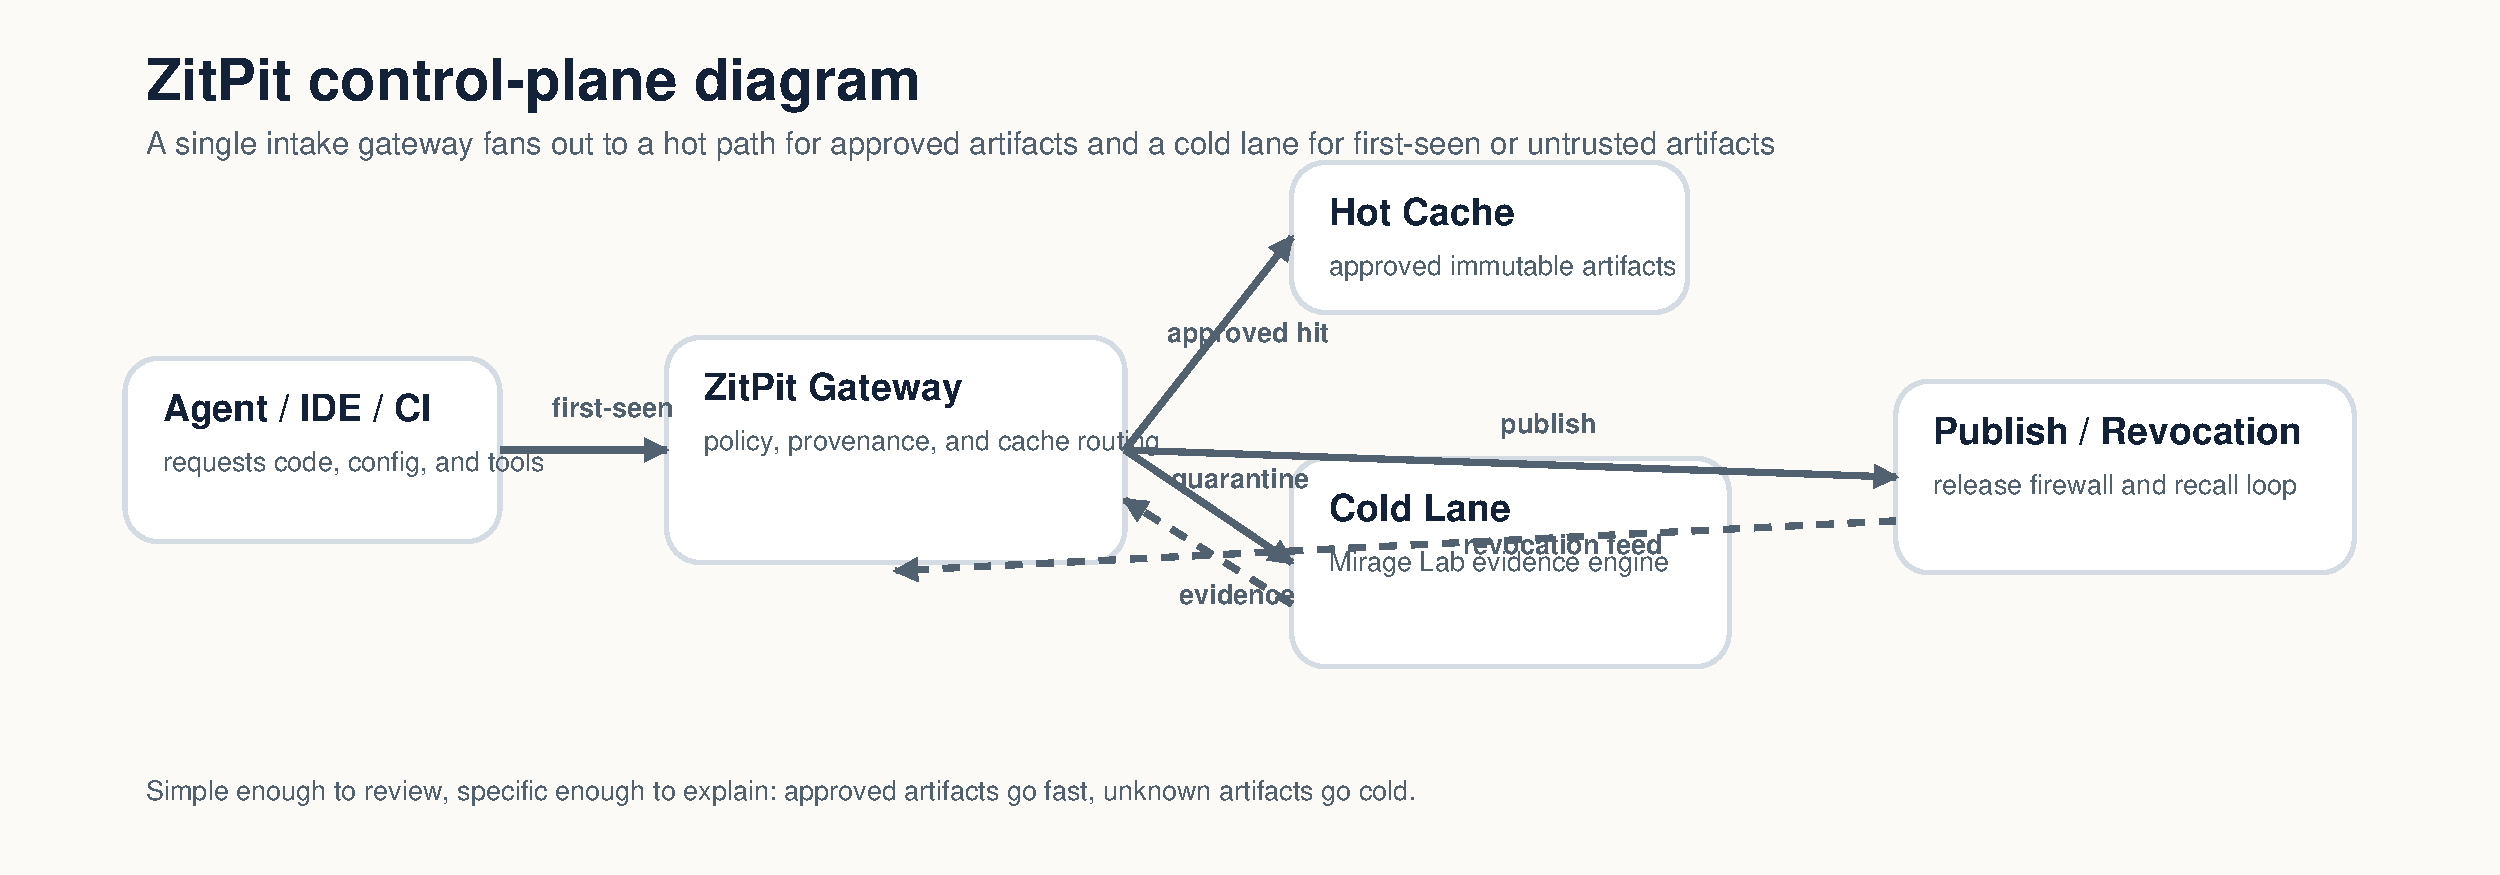
\includegraphics[width=0.85\textwidth]{figures/network.pdf}
\caption{Simplified \product{} control plane. Agents, IDEs, and CI runners enter through a single intake gateway. Approved immutable artifacts remain on the fast path through local cache and hot cache. First-seen or sensitive artifacts fall to a cold lane where Mirage Lab gathers evidence before promotion, expiry, or revocation updates policy.}
\label{fig:network}
\end{figure*}

\subsection{Acquire}

All mediated intake resolves through a gateway that attempts to map a request onto an immutable object identity. For Git this may be a resolved commit behind a smart-HTTP request. For package ecosystems it may be a tarball digest, wheel identity, or crate digest. For workflow references it should be a full commit SHA. Mutable selectors such as floating tags, branch heads, and \texttt{latest} are treated as policy exceptions rather than ambient trust.

\subsection{Build}

The build stage separates fetching bytes from running code. This distinction matters because many developer tools blur the two together. npm lifecycle hooks, Python source distributions, Rust build scripts, and shell installers all have paths where download and execution happen in one command \cite{npmPackageJson2026,cargoBuildScripts2026}. In \product{}, first-seen or policy-sensitive objects are routed into a cold lane before those execution surfaces touch a protected host.

\subsection{Execute}

Execution rights are capability-scoped rather than binary. A useful policy can say ``the bytes may be fetched'' without also saying ``the code may run in a developer shell with secrets available.'' This is especially important for repo-open surfaces. Workspace configuration, MCP definitions, devcontainers, and startup hooks are treated as supply-chain input because they can cause execution simply by opening a project \cite{anthropicMcp2026,anthropicDevcontainer2026}.

\subsection{Publish}

The publish stage is logically separate because producer-side release failures are different from consumer-side intake attacks. A release firewall can validate exact outbound artifacts, compare them against expected provenance or workflow identity, and block accidental leaks before publication. That control belongs in the larger \product{} story, but it should not be confused with the core intake claim made in this paper.

\subsection{Mirage Lab and policy evidence}

Mirage Lab is the cold-lane evidence engine. It is intentionally not treated as a magic safety oracle. A quiet sandbox run does not prove software is safe. What Mirage Lab does provide is evidence: network attempts, file-system activity, process spawning, unexpected tool launches, and other signals that can support promotion, blocking, expiry, or recall decisions. The stronger claim is therefore not ``the sandbox said it was safe.'' The stronger claim is ``the code never executed on the protected host before policy and evidence existed.''

\section{Artifact Intake and Governed Execution}

\subsection{Security invariants}

Three invariants carry most of the design:
\begin{enumerate}
\item \textbf{First-seen code is a policy event.} Unknown third-party code does not silently inherit execution rights.
\item \textbf{Immutable identity comes before execution.} Digest resolution, pinning, or equivalent immutable identity should precede trust.
\item \textbf{The safe path is the fast path.} Approved immutable artifacts should be easier and faster to consume than unmanaged public fetch.
\end{enumerate}

These invariants are intentionally stronger than ``we collect hashes'' and intentionally narrower than ``we solve supply-chain security.'' They are the basis for both the performance argument and the honesty of the paper.

\subsection{Capability-scoped policy}

\product{} uses capability-scoped verdicts rather than coarse allow-or-block decisions. Representative verdicts include \texttt{FETCH\_ONLY}, \texttt{BUILD\_NO\_NETWORK}, \texttt{TEST\_NO\_SECRETS}, \texttt{RUN\_DEV}, \texttt{RUN\_CI}, and \texttt{BLOCKED}. This makes it possible to express policy that matches real workflows: a first-seen package may be fetched and detonated in a controlled lane without being allowed to execute on a developer machine.

\begin{table}[t]
\caption{Representative capability-scoped verdicts}
\label{tab:verdicts}
\centering
\footnotesize
\setlength{\tabcolsep}{4pt}
\begin{tabular}{p{0.27\columnwidth} p{0.62\columnwidth}}
\toprule
\textbf{Verdict} & \textbf{Meaning} \\
\midrule
\texttt{FETCH\_ONLY} & Download allowed, host execution denied pending more trust. \\
\texttt{BUILD\_NO\_NETWORK} & Build allowed only in a controlled lane without network egress. \\
\texttt{TEST\_NO\_SECRETS} & Test execution allowed in an isolated environment without sensitive material. \\
\texttt{RUN\_DEV} & Approved for normal developer use on protected hosts. \\
\texttt{RUN\_CI} & Approved for CI execution under policy and freshness requirements. \\
\texttt{BLOCKED} & Denied pending operator intervention, expiry, or recall. \\
\bottomrule
\end{tabular}
\end{table}

\subsection{Trust inputs}

Digest equality matters because it creates immutable identity, but identity is not provenance. \product{} is designed to consume several stronger trust signals when available: TUF-style freshness and anti-rollback semantics \cite{tufDocs2026,tufPaper2016}, Sigstore-style identity-bound signing and transparency logs \cite{sigstoreDocs2026}, in-toto attestations for build-step integrity \cite{intotoDocs2026,intotoPaper2019}, SLSA provenance expectations \cite{slsaDocs2026}, GitHub artifact attestations \cite{githubArtifactAttestations2026}, and ecosystem-native trusted publishing such as npm trusted publishers \cite{npmTrustedPublishing2026}. An approval record therefore needs more than a hash; it needs origin, freshness, evidence, and revocation state.

\subsection{Deployment and operator experience}

An intake control only survives in practice if it is easy to turn on and easy to keep on. \product{} therefore exposes a short setup path for a local operator:

\begin{lstlisting}[language=bash,caption={Current local setup path used in the repository quickstart.},label={lst:install}]
cargo run -p xtask -- demo setup
ssh zitpit
cargo run -p zitpit-tui
\end{lstlisting}

The first command prepares the local environment, prints a safe SSH stanza, and starts the mediated path. The second enters the protected shell. The third opens the operator TUI that shows policy decisions, cold-lane detonation state, and approval history. This matters because a practical firewall for AI-assisted development has to feel like an accelerator, not a lecture.

\begin{figure*}[t]
\centering
\subfloat[Cursor-side developer workflow under mediated intake.]{
  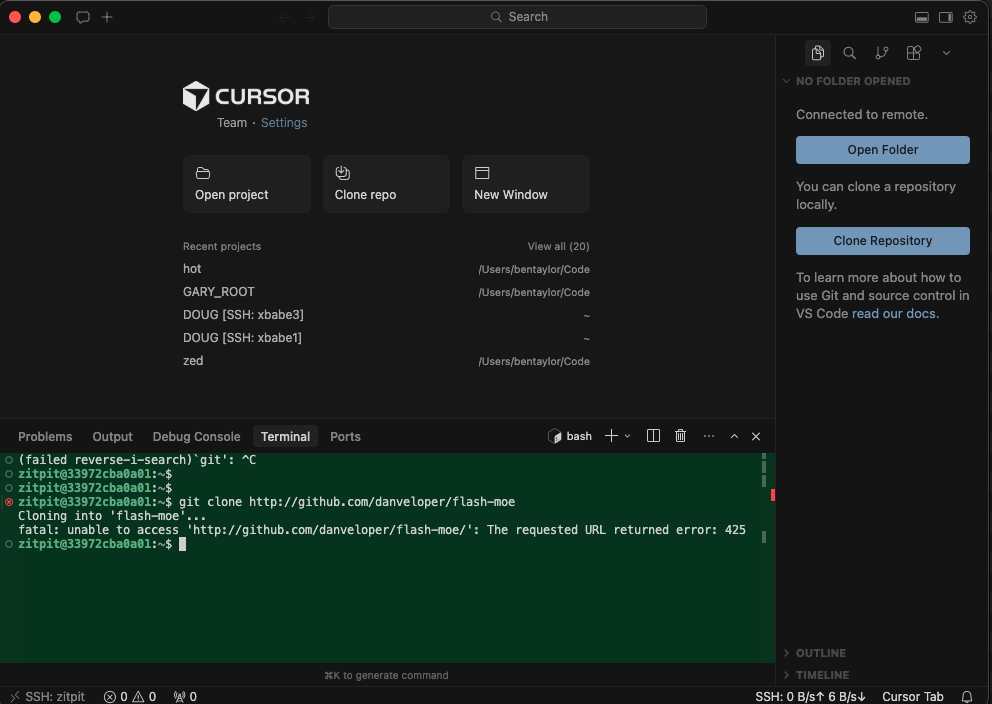
\includegraphics[width=0.485\textwidth]{figures/cursor_zitt.png}
  \label{fig:cursor}
}
\hfill
\subfloat[Operator view in the ZitPit TUI.]{
  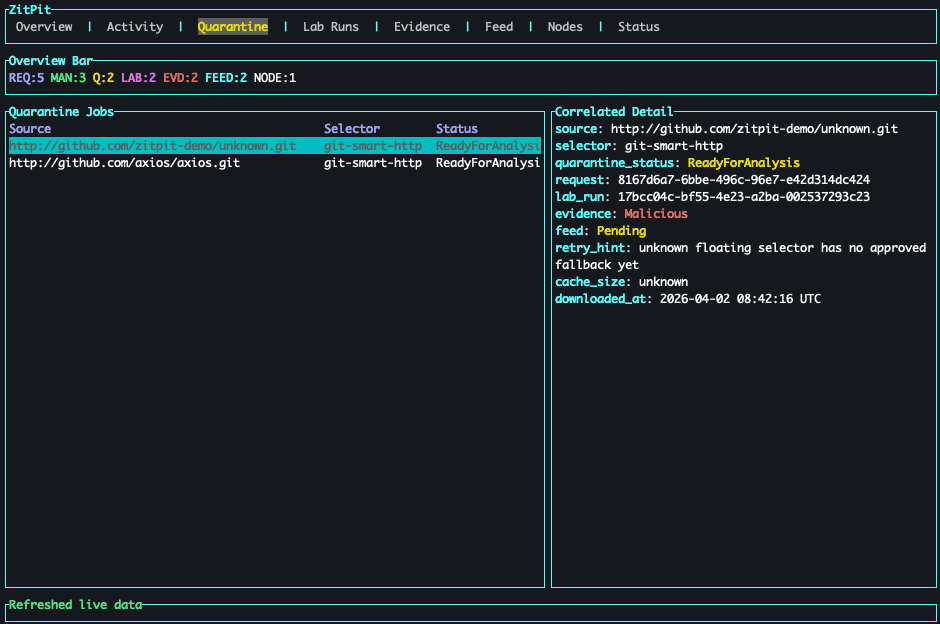
\includegraphics[width=0.485\textwidth]{figures/zitt_TUI.png}
  \label{fig:tui}
}
\caption{Usability matters because developers and agents bypass slow or opaque controls. \product{} is designed to keep the mediated path close to normal developer ergonomics while surfacing enough policy and evidence for operators to intervene when needed.}
\label{fig:screens}
\end{figure*}

\section{Performance and Coverage Evaluation}

\begin{figure*}[t]
\centering
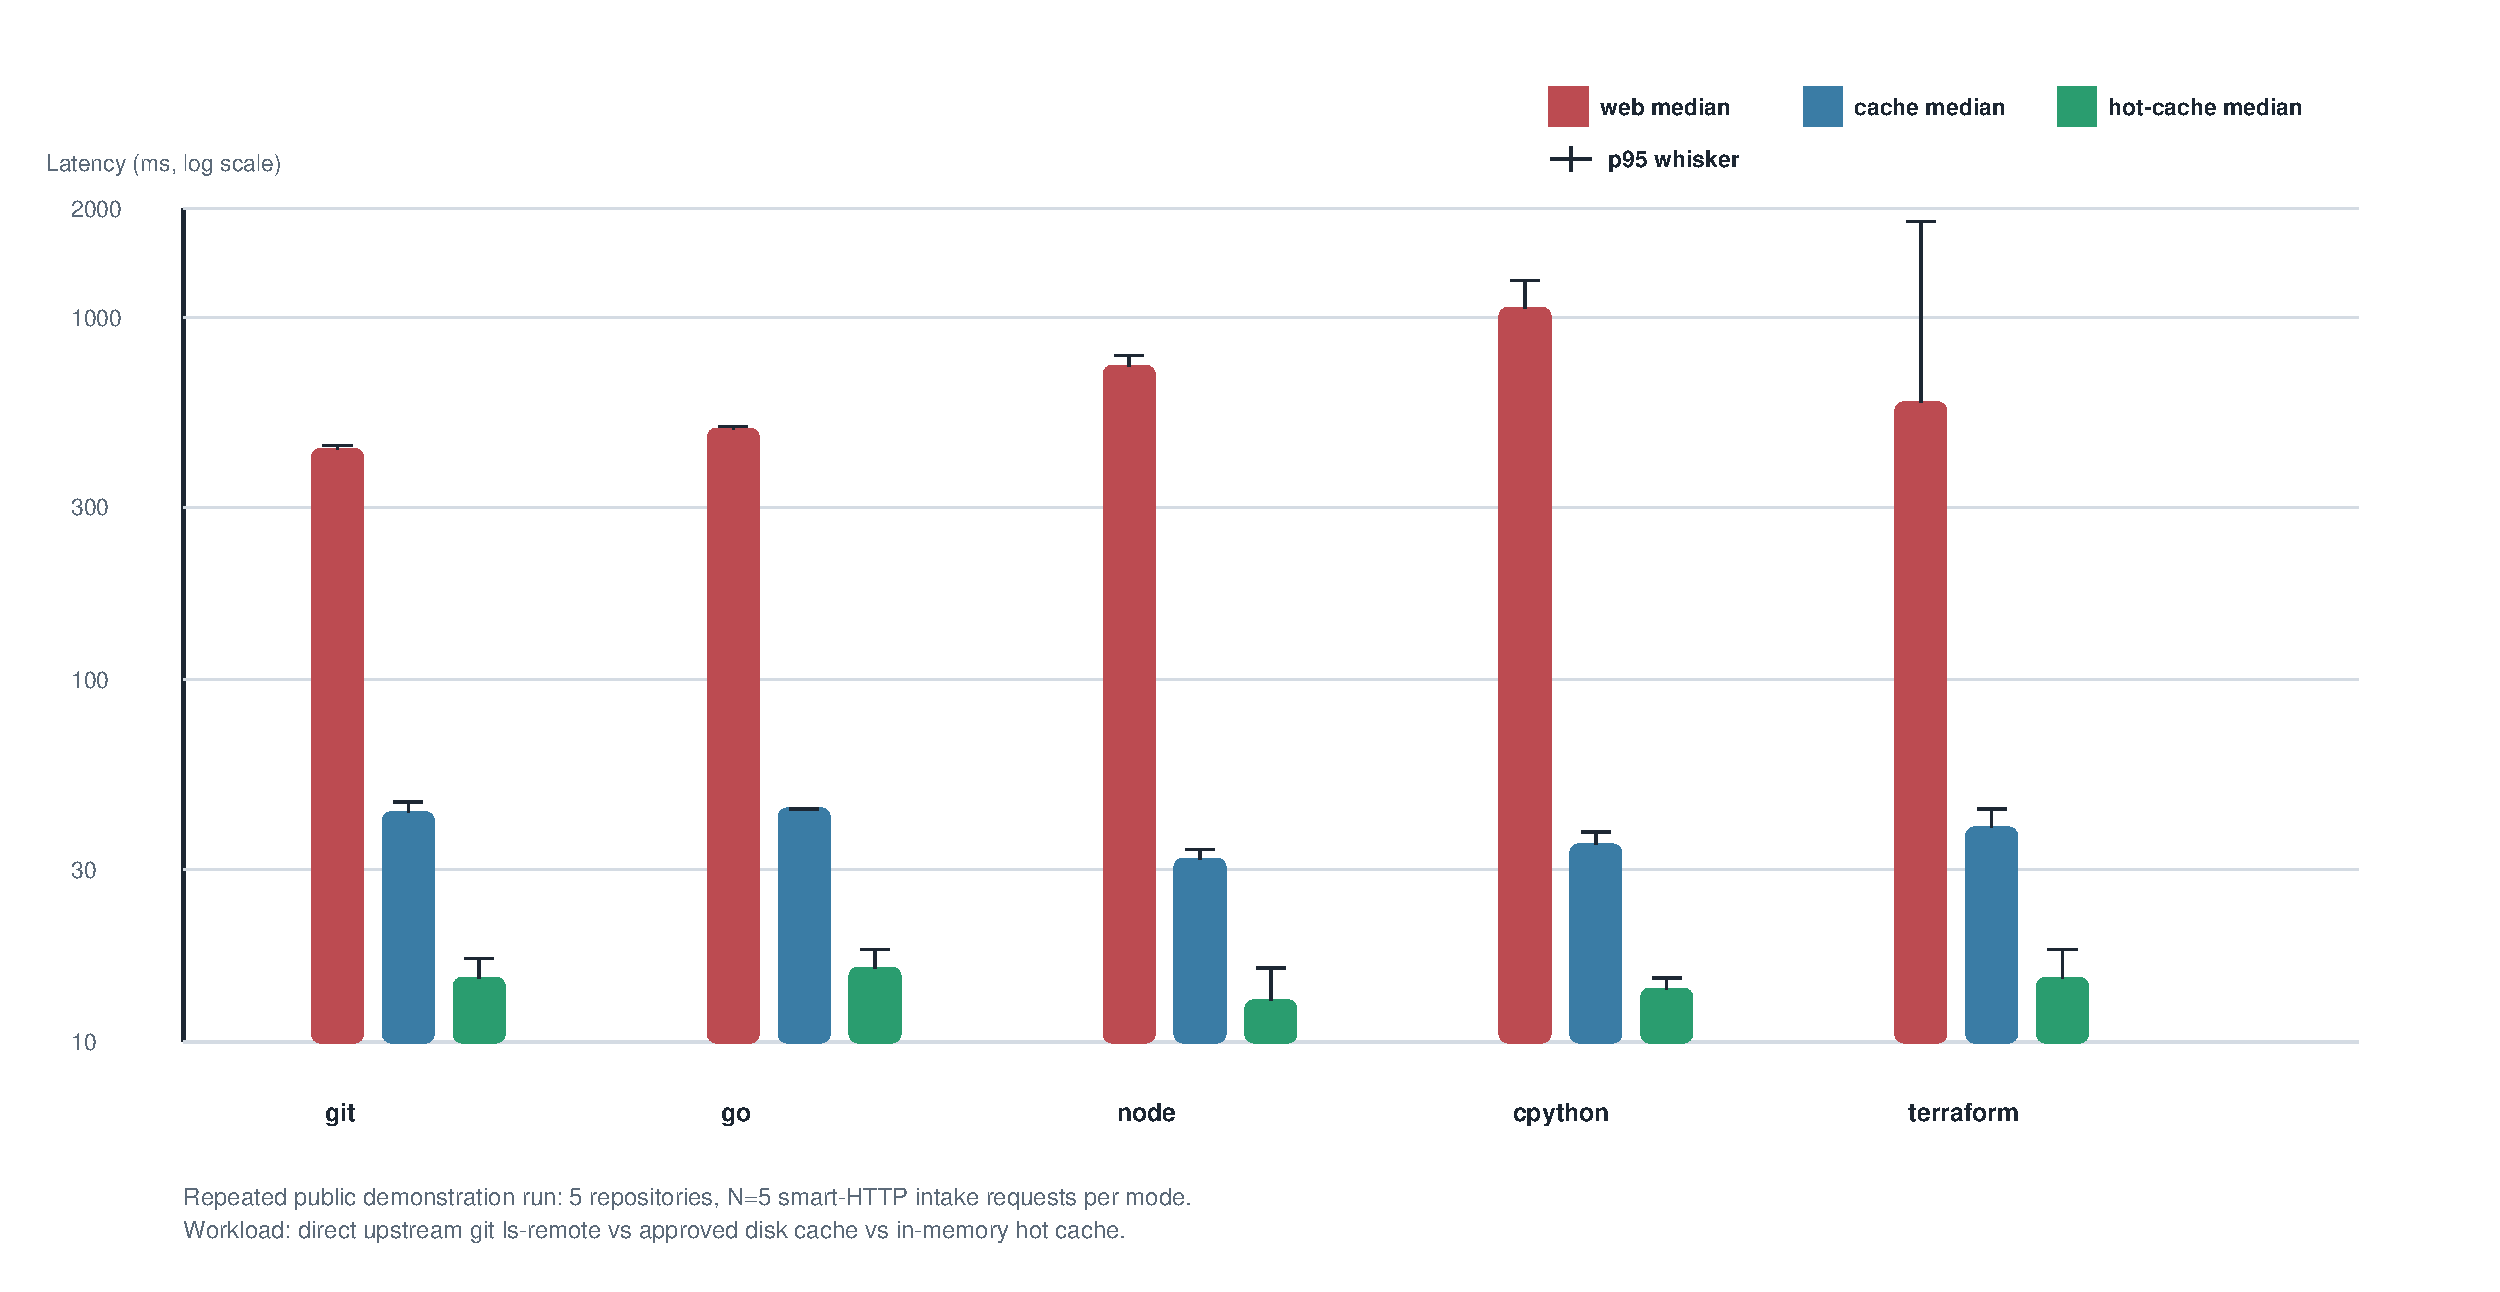
\includegraphics[width=0.88\textwidth]{figures/speedup.pdf}
\caption{Current five-repository demonstration run for the Git smart-HTTP intake path. The governed path is already faster for approved immutable artifacts: direct upstream requests took 413--821~ms, disk-cache hits 30--34~ms, and hot-cache hits 14--16~ms.}
\label{fig:speedup}
\end{figure*}

The public benchmark matrix is the source of truth for what \product{} can honestly claim. Today that matrix includes Git intake, npm install-time behavior, Python startup and sdist paths, Rust \texttt{build.rs}, GitHub Actions mutability, raw shell installer fetches, repo-open workspace surfaces, and benign controls across the same families \cite{zitpitBenchmarkMatrix2026}. The matrix is intentionally public because credibility depends on showing the current claim boundary rather than hiding it.

\subsection{Git intake performance}

The current implementation already supports a narrow but important claim: the governed path can be faster than direct upstream access for approved immutable artifacts. The benchmark harness records the smart-HTTP intake request path for five recognizable public repositories: \texttt{git}, \texttt{go}, \texttt{node}, \texttt{cpython}, and \texttt{terraform}. For each repository, the harness records three modes: direct upstream request (\texttt{web}), approved disk-cache hit (\texttt{cache}), and approved in-memory hit (\texttt{hot-cache}) \cite{zitpitBench2026}.

\begin{table}[t]
\caption{Five-repository public demonstration snapshot}
\label{tab:gitbench}
\centering
\footnotesize
\begin{tabular}{lrrrr}
\toprule
\textbf{Repo} & \textbf{Web} & \textbf{Cache} & \textbf{Hot} & \textbf{Hot speedup} \\
\midrule
git & 413 & 34 & 15 & 27.5x \\
go & 479 & 30 & 16 & 29.9x \\
node & 697 & 31 & 14 & 49.8x \\
cpython & 821 & 31 & 15 & 54.7x \\
terraform & 755 & 33 & 16 & 47.2x \\
\bottomrule
\end{tabular}
\end{table}

In the current snapshot, direct upstream requests took 413--821~ms, disk-cache hits took 30--34~ms, and hot-cache hits took 14--16~ms. The median values are 697~ms for \texttt{web}, 31~ms for \texttt{cache}, and 15~ms for \texttt{hot-cache}. The sample count in this snapshot is modest (\(N=1\) per repository), so the result should be read as a public demonstration rather than a definitive latency study. Even with that limitation, the operational message is already visible: policy mediation does not have to be the slow path.

\subsection{Coverage beyond Git}

Git matters because it is the cleanest performance story in the current codebase, but the system is not framed as Git-only. Public battle packs and benchmark families now cover npm install scripts, Python startup and build paths, Cargo build scripts, Go module control paths, GitHub Actions mutability, direct shell downloads, and workspace-open surfaces such as \texttt{.mcp.json} and devcontainers \cite{zitpitBenchmarkMatrix2026}. This broader coverage matters because the modern intake problem is heterogeneous. An artifact firewall that only sees \texttt{git clone} misses too much of the real execution surface.

\subsection{Reproducibility and public evidence}

The evidence supporting this paper is intentionally inspectable. The benchmark matrix, raw timing JSON, battle packs, figure generator, LaTeX sources, and publication figures live in the same repository as the system code \cite{zitpitBenchmarkMatrix2026,zitpitBench2026}. That transparency matters for two reasons. First, it makes the claim boundary auditable. Second, it gives the open source community a direct way to challenge the system with new adapters, harder workloads, and tighter measurements without having to reverse-engineer a closed benchmark harness.

\section{Limitations and Concerns}

The paper is strongest when its limits are explicit. First, \product{} does not make trusted maintainers harmless. If a trusted publisher ships malicious code under a valid identity, an intake firewall still needs stronger provenance policy, revocation, or external intelligence to react. Second, consumer-side intake mediation is not the same thing as producer-side release hygiene. A packaging leak, source-map exposure, or wrong-registry publish needs publish controls, not just inbound mediation. Third, unsupported ingress paths must be called out honestly. If a tool fetches code outside the mediated path, the right claim is ``unsupported'' rather than ``secure enough.''

Fourth, Mirage Lab evidence is informative but not definitive. Dynamic analysis can miss dormant logic, trigger-dependent behavior, or environment-specific payloads. Treating sandbox silence as proof of safety would undercut the rest of the paper. Finally, the current public performance snapshot is intentionally small. The Git timing data is a reproducible proof point, but it is not yet a full cross-ecosystem, multi-run latency study. The right next step is broader measurement, not bigger claims.

\section{Community Roadmap}

The project is open source because the benchmark boundary, battle packs, and policy adapters should improve in public. The most useful community extensions are concrete:
\begin{itemize}
\item broader ecosystem adapters for package managers, OCI artifacts, and raw download paths;
\item stronger provenance integrations for Sigstore, GitHub artifact attestations, in-toto, and SLSA;
\item publish-side controls that prevent accidental release leaks and workflow drift before outbound publication;
\item wider benchmark programs with repeated runs, percentile reporting, and more realistic CI and agent workloads;
\item deeper agent-native enforcement for IDEs, MCP tooling, and repo-open policy hooks.
\end{itemize}

This roadmap is intentionally evolutionary rather than theatrical. The value of community support is not that it changes the core claim. The value is that it lets the project widen coverage, sharpen evidence, and make the mediated path useful across more real-world toolchains without abandoning the central design contract.

\section{Related Work}

\product{} sits at the intersection of several established lines of work. TUF provides the reference model for freshness, delegation, and anti-rollback semantics in update systems \cite{tufDocs2026,tufPaper2016}. in-toto focuses on recording and verifying build-step integrity \cite{intotoDocs2026,intotoPaper2019}. SLSA provides a vocabulary for software provenance guarantees \cite{slsaDocs2026}. Sigstore supplies identity-bound signing and transparency infrastructure for modern software publication \cite{sigstoreDocs2026}. GitHub artifact attestations and npm trusted publishing are practical examples of mainstream provenance and identity work entering everyday developer tooling \cite{githubArtifactAttestations2026,npmTrustedPublishing2026}.

\product{} also draws from a long tradition of sandboxing and deception systems, but with a deliberate shift in emphasis. The Mirage Lab is not the root trust primitive; it is an evidence engine attached to a policy gate. That ordering reflects both the feedback captured during the project's public review and the operational reality that governed execution boundaries matter more than theatrical detonation if the goal is to protect real developer and CI hosts.

\section{Conclusion}

\product{} starts from a practical observation about AI-assisted development: the interval between ``discover external code'' and ``execute external code'' is collapsing toward zero. That collapse changes the default security problem. What used to be a repository review problem is now a systems problem spanning registries, workflow engines, raw downloads, and repo-open configuration. The right response is not a grand claim about solving software supply-chain security forever. The right response is a narrow and enforceable contract: first-seen external code becomes a policy event before it becomes execution on a protected host, and approved immutable artifacts are served fast enough that developers and agents have less reason to bypass the gate.

The current implementation already demonstrates the beginning of that contract. In the public Git intake benchmark, approved cache and hot-cache paths are materially faster than direct upstream access. The codebase and benchmark suite already reach beyond Git into package-manager, workflow, shell, and workspace surfaces. The paper's broader argument is therefore not that \product{} is finished. It is that an artifact firewall for agentic software supply chains is now both necessary and technically tractable, and that an open community can extend the evidence and coverage surface without sacrificing honesty about what the system does and does not yet prove.

\balance
\bibliographystyle{IEEEtran}
\bibliography{references}

\end{document}
